\chapter{NEST - A short tutorial\label{app:nest}}

\graphicspath{{figs/appendices/}}



NEST (NEural Simulation Tool, \citeN{Gewaltig:NEST}) is a simulation environment developed by the NEST Initiative, capable of running simulations of large networks of point neurons. NEST is open source and can be downloaded free of charge from \href{http://nest-initiative.org}{nest-initiative.org}. A brief introduction is given here. This section is based on the NEST tutorial by \citeN{gewaltig2012nest} and the NEST Topology User Manual by \citeN{plesser2012topo}. It mainly describes the functions implementing the connection algorithms tested in this thesis. A Python interface, PyNEST \shortcite{Eppler:PyNEST}, is available, and will be used here. Version 2.2.0 of NEST is used.
To import the PyNEST module into Python we use the following command.
\begin{lstlisting}
import nest
\end{lstlisting}

The concepts of \emph{nodes} and \emph{connections} described earlier are used in NEST. {\bf Nodes} can be neurons, devices, or sub-networks. The neurons are either point-neurons (neurons with a single compartment) or neurons with a small number of compartments. They can be based on one of the many built-in neuron models, some of which are listed in Table \ref{tab:neur_mod}. The default parameters of each of these models can be modified. Due to NEST's modular architecture, researchers can also create their own models from scratch. 

\begin{table}
\begin{tabularx}{\textwidth}{| l | X |}
\hline
\bf{Name} & \bf{Description} \\ \hline
aeif\_cond\_alpha & Conductance based exponential integrate-and-fire neuron model according to \citeN{brette2005adaptive}. \\ \hline
% aeif\_cond\_exp & desc \\ \hline
ginzburg\_neuron & Binary stochastic neuron with sigmoidal activation function. \\ \hline
% hh\_cond\_exp\_traub & Hodgin Huxley based model, Traub modified. \\ \hline
hh\_psc\_alpha & Spiking neuron using the Hodkin-Huxley formalism. \\ \hline
ht\_neuron & Neuron model after \citeN{hill2005modeling}. \\ \hline
iaf\_cond\_alpha & Simple conductance based leaky integrate-and-fire neuron model. Post-synaptic change 
of conductance modelled by an alpha function.\\ \hline
% iaf\_cond\_alpha\_mc & desc \\ \hline
iaf\_cond\_exp & Simple conductance based leaky integrate-and-fire neuron model. Post-synaptic change 
of conductance modeled by an exponential function. \\ \hline
% iaf\_cond\_exp\_sfa\_rr & desc \\ \hline
iaf\_neuron & Leaky integrate-and-fire model with alpha-function shaped synaptic currents. \\ \hline
% iaf\_psc\_alpha & desc \\ \hline
% iaf\_psc\_alpha\_canon & desc \\ \hline
% iaf\_psc\_alpha\_presc & desc \\ \hline
% iaf\_psc\_delta & desc \\ \hline
% iaf\_psc\_delta\_canon & desc \\ \hline
% iaf\_psc\_exp & desc \\ \hline
% iaf\_psc\_exp\_ps & desc \\ \hline
% iaf\_tum\_2000 & desc \\ \hline
izhikevich & Implementation of the simple spiking neuron model introduced by \citeN{izhikevich2003simple}. \\ \hline
mat2\_psc\_exp & Non-resetting leaky integrate-and-fire neuron model with exponential PSCs and adaptive threshold. \\ \hline
parrot\_neuron & Neuron that repeats incoming spikes. \\ \hline
% parrot\_neuron\_ps & desc \\ \hline
pp\_psc\_delta & Point process neuron with leaky integration of delta-shaped PSCs. \\ \hline
sli\_neuron & The sli\_neuron is a model whose state, update and calibration can be defined in SLI. \\ \hline
% subnet & desc \\ \hline
% topology\_layer\_free & desc \\ \hline
% topology\_layer\_free\_3d & desc \\ \hline
% topology\_layer\_grid & desc \\ \hline
%topology\_layer\_grid\_3d & desc \\ \hline
\end{tabularx} 
\caption[Neuron models in NEST]{A few of the neuron models available in NEST.}
\label{tab:neur_mod}
\end{table}

Devices are nodes used to either stimulate or measure the activity of neurons. Some of the available devices are listed in Table \ref{tab:dev_mod}. Sub-networks (or subnets) are nodes who themselves are comprised of multiple nodes. Subnets can also be created inside other subnets. Using nested subnets we can create complex hierarchical structures of neurons with as many levels as we want. 

The Python code below will create a neuron of type ``iaf\_neuron'', using the default parameters for the model. 
\begin{lstlisting}
neuron1 = nest.Create('iaf_neuron')
\end{lstlisting}
Every node created is assigned number, called a global identifier (GID). This number is returned and assigned to the variable called \inline{neuron1}.
To create a neuron with some non-default parameters, say, the threshold potential $V_{\text{th}}$ and the reset potential $V_{\text{reset}}$, the code will look as follows. 
\begin{lstlisting}
neuron2 = nest.Create('iaf_neuron', 
                      params={'V_th': -50.0, 'V_reset': -65.0})
\end{lstlisting}
To create many identical nodes, the desired number of nodes is passed to \inline{Create} as the second argument. In the following code 1,000 neurons are created, and the GIDs for all the neurons are stored as a list named \inline{neurons}.
\begin{lstlisting}
neurons = nest.Create('iaf_neuron', 1000)
\end{lstlisting}

\begin{table}
\begin{tabularx}{\textwidth}{| l | X |}
\hline
\bf{Name} & \bf{Description} \\ \hline
ac\_generator & This device produce an ac-current. \\ \hline
correlation\_detector & Device for evaluating cross correlation between two spike sources \\ \hline
dc\_generator & The DC-Generator provides a constant DC input to the connected node. \\ \hline
gamma\_sup\_generator & Simulate the superimposed spike train of a population of gamma process. \\ \hline
% mip\_generator & desc \\ \hline
multimeter & Device to record analog data from neurons. \\ \hline
noise\_generator & Device to generate Gaussian white noise current. \\ \hline
poisson\_generator & Simulate neuron firing with Poisson processes statistics. \\ \hline
% poisson\_generator\_ps & desc \\ \hline
% ppd\_sup\_generator & desc \\ \hline
% pulsepacket\_generator & desc \\ \hline
% smp\_generator & desc \\ \hline
spike\_detector & Device for detecting single spikes. \\ \hline
spike\_generator & A device which generates spikes from an array with spike-times. \\ \hline
% step\_current\_generator & desc \\ \hline
voltmeter & Device to record membrane potentials from neurons. \\ \hline
% volume\_transmitter & desc \\ \hline
\end{tabularx}
\caption[Devices in NEST]{Some of the devices available in NEST.}
\label{tab:dev_mod}
\end{table}

{\bf Connections} in NEST can represent synapses between neurons, but can also be connections from neurons to other types of nodes (devices and subnets). All connections are \emph{directed}, \emph{weighted} and \emph{delayed}. Directed means information travels in one direction. Weighted means the strength of connections can be varied. Delayed means it takes time for information to travel from one node to a connected node.

To manually connect one pair of nodes using the default synapse model ``static\_synapse'' with the default weight of $1.0$ and the default delay of $1.0$ milliseconds we can use the \inline{Connect} function:
\begin{lstlisting}
nest.Connect(neuron1, neuron2)
\end{lstlisting}
To use a weight of $-1.5$ (negative weights means the connection will be inhibitory), a delay of $0.5$ ms, and the synapse model ``tsodyks\_synapse'', we pass some extra arguments to \inline{Connect} as follows.
\begin{lstlisting}
nest.Connect(n1, n2, -1.5, 0.5, model='tsodyks_synapse')
\end{lstlisting}
Table \ref{tab:syn_mod} lists some of the synapse models in NEST. Several synapse models with short-term and long-term plasticity are available.

\begin{table}
\begin{tabularx}{\textwidth}{| l | X |}
\hline
\bf{Name} & \bf{Description} \\ \hline
cont\_delay\_synapse & Synapse type for continuous delays. \\ \hline
ht\_synapse & Synapse with depression after \citeN{hill2005modeling}. \\ \hline
static\_synapse & Synapse type for static connections. \\ \hline
% static\_synapse\_hom\_wd & desc \\ \hline
stdp\_dopamine\_synapse & Synapse type for dopamine-modulated spike-timing dependent plasticity. \\ \hline
% stdp\_pl\_synapse\_hom & desc \\ \hline
stdp\_synapse & Synapse type for spike-timing dependent plasticity. \\ \hline
% stdp\_synapse\_hom & desc \\ \hline
% tsodyks2\_synapse & desc \\ \hline
tsodyks\_synapse & Synapse type with short term plasticity. \\ \hline
\end{tabularx}
\caption[Synapse models in NEST]{Some of the synapse models available in NEST.}
\label{tab:syn_mod}
\end{table}

\inline{Connect} can also be used to create many one-to-one connections between two lists of nodes. However, if we wish to make connections that are more \linebreak complex than simple one-to-one connections, such as convergent and \linebreak divergent connections, several other functions are available. One example is \linebreak\inline{RandomConvergentConnect}. The code snippet below first defines three \linebreak variables $N_\text{s}$, $N_\text{t}$ and $C$. It then creates $N_\text{s}$ neurons, which will serve \linebreak as \emph{source} neurons, and $N_\text{t}$ \emph{target} neurons. It then connects them using \linebreak \inline{RandomConvergentConnect}. 
\begin{lstlisting}
N_s = 10
N_t = 10
C = 3
source_neurons = nest.Create('iaf_neuron', N_s)
target_neurons = nest.Create('iaf_neuron', N_t)
nest.RandomConvergentConnect(source_neurons, target_neurons, C)
\end{lstlisting}
The function call
\begin{lstlisting}
nest.GetConnections(source_neurons)
\end{lstlisting}
will return the resulting connections. \inline{RandomConvergentConnect} considers each node in the second list (\inline{target_neurons}) in turn, and connects $C$ randomly chosen nodes from the first list (\inline{source_neurons}). Hence, the target nodes will all have an in-degree (number of incoming connections) equal to $C$, whereas the source nodes might have different out-degrees. Note that two or more connections (multapses) can be drawn between the same pair of nodes. 

A similar function, \inline{RandomDivergentConnect}, works in very much the same way, but it iterates over the \emph{source} nodes instead of the target nodes, and draws random nodes from the \emph{targets} instead of the sources. As a result, the source nodes will now all have the same out-degree $C$, while the in-degrees of the target nodes will vary. An example of a random divergent network was shown in Figure \ref{fig:rdc_example_intro}.

After having created all nodes and connected them, the simulation can be started with the \inline{Simulate} function. \inline{Simulate} only takes one argument; the number of milliseconds to simulate. The following example, borrowed from \citeN{gewaltig2012nest}, is a simple simulation script. A neuron receives stimuli (events) from one AC generator and two poisson generators. A voltmeter is also connected to the neuron to record the membrane potential. The simulation is run for 1,000 ms, and a plot of the membrane potential as a function of time is displayed.

\begin{lstlisting}
import nest
import nest.voltage_trace
neuron = nest.Create('iaf_neuron')
sine = nest.Create('ac_generator', 1, 
                   {'amplitude': 100.0, 'frequency': 2.0})
noise = nest.Create('poisson_generator', 2, 
                    [{'rate': 70000.0}, {'rate': 20000.0}])
voltmeter = nest.Create('voltmeter', 1, {'withgid': True})
nest.Connect(sine, neuron)
nest.Connect(voltmeter, neuron)
nest.ConvergentConnect(noise, neuron, [1.0, -1.0], 1.0)
nest.Simulate(1000.0)
nest.voltage_trace.from_device(voltmeter)
\end{lstlisting}



\subsubsection{Spatially structured networks and the NEST Topology module}

The simulation of spatially structured networks is increasingly a popular tool. A spatially structured network is a network where connection probabilities and -properties are determined by the spatial position of the nodes. With NEST, such networks can be created easily using the NEST Topology module \shortcite{plesser2009specification,plesser2012topo}. 

To use NEST Topology, the module has to be imported as show below. For convenience it is given the shorthand name ``topo''.
\begin{lstlisting}
import nest
import nest.topology as topo
\end{lstlisting}
In Topology, nodes are placed on \emph{layers}. Layers are similar to subnets, but with extra information about the spatial position of each node. The term ``layer'' often refers to a two-dimensional structure, but layers in NEST Topology can be both two- and three-dimensional. They are either grid-based or free. In \emph{grid-based layers}, nodes are placed on a Cartesian grid, while on \emph{free layers}, nodes can be placed at arbitrary locations. The code below will create a simple two-dimensional grid-based layer. 
\begin{lstlisting}
layer_specs = {'elements': 'iaf_neuron', 
               'rows': 10, 'columns': 10, 'extent': [2.0, 2.0]}
layer = topo.CreateLayer(layer_specs)
\end{lstlisting}
First a dictionary, \inline{layer_specs}, is created, containing specifications for the layer. The node type is set to ``iaf\_neuron''. The \inline{rows} and \inline{columns} entries specify the number of desired rows and columns of neurons, and \inline{extent} is the size of the layer. Additional parameters can be included, such as the $x$ and $y$ position of the center of the layer (default is (0, 0)). The layer is assigned a GID, which is returned by \inline{CreateLayer} and assigned to the variable \inline{layer}.

To create a \emph{free} layer, the position of every node must be passed to\linebreak \inline{CreateLayer}. If a list of positions is given, a node will be created at each. In the example below, three nodes are positioned on a two-dimensional layer. 
\begin{lstlisting}
pos = [[-0.3, 0.3], [0.4, 0.2], [0.0, -0.4]]
layer = topo.CreateLayer({'elements': 'iaf_neuron', 
                          'positions': pos})
\end{lstlisting}
Here the extent is not specified, so the layer will have the default extent of $1.0 \times 1.0$. 

To place a larger number of neurons at pseudorandom locations, we have to import and use a pseudorandom number generator (PRNG), such as the one supplied with \inline{numpy}. Here, 1,000 neurons are uniformly distributed over the layer:
\begin{lstlisting}
import numpy as np
x = np.random.uniform(-0.5, 0.5, 1000)
y = np.random.uniform(-0.5, 0.5, 1000)
pos = zip(x, y)
l = topo.CreateLayer({'elements': 'iaf_neuron', 
                      'positions': pos})
topo.PlotLayer(l)
\end{lstlisting}
The last line will display a plot of all the nodes on the layer, similar to the one in Figure \ref{fig:free_layer}.
\begin{figure}[h]
  \centering
  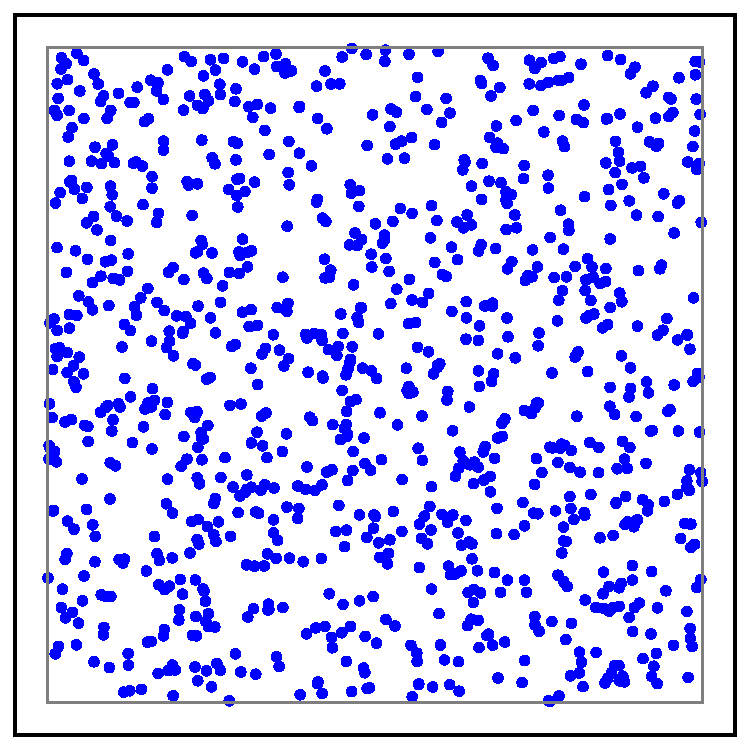
\includegraphics[width=0.6\textwidth]{FreeLayer.pdf}
  \caption[Example of free two-dimensional layer]{A free layer with 1,000 nodes. $x$ and $y$ positions are drawn pseudorandomly from~$\mathcal{U}(-0.5, 0.5)$.}
  \label{fig:free_layer}
\end{figure}
To create a three-dimensional layer we simply add a third component to the node positions.
\begin{lstlisting}
import numpy as np
x = np.random.uniform(-0.5, 0.5, 1000)
y = np.random.uniform(-0.5, 0.5, 1000)
z = np.random.uniform(-0.5, 0.5, 1000)
pos = zip(x, y, z)
l = topo.CreateLayer({'elements': 'iaf_neuron', 
                      'positions': pos})
topo.PlotLayer(l)
\end{lstlisting}
The result is seen in Figure \ref{fig:free_3D_layer}.
\begin{figure}[h]
  \centering
  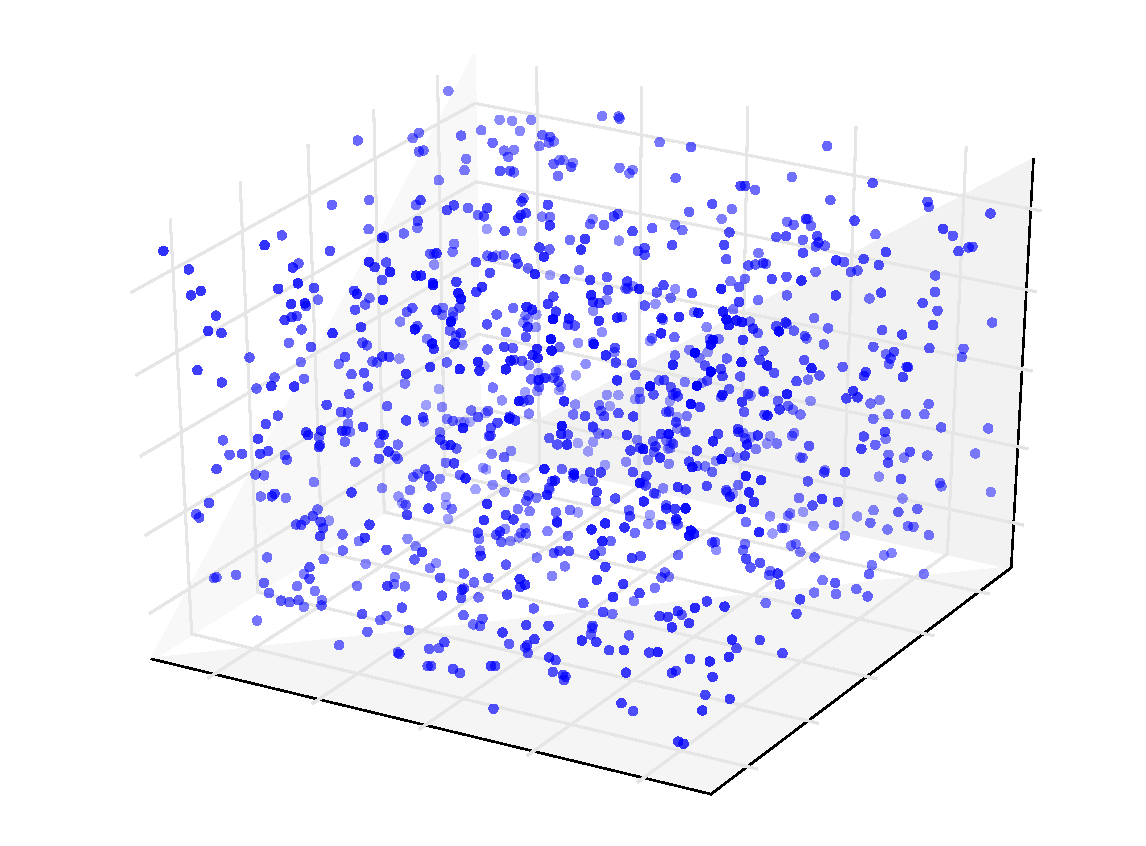
\includegraphics[width=0.8\textwidth]{TopologyExample3D.pdf}
  \caption[Example of free three-dimensional layer]{A free three-dimensional layer with 1,000 nodes, where $x$, $y$, and $z$ positions are drawn pseudorandomly from~$\mathcal{U}(-0.5, 0.5)$.}
  \label{fig:free_3D_layer}
\end{figure}

For small layers, a large fraction of the nodes will be close to the edge and therefore have fewer neighboring nodes. This might have an undesired effect on the simulation. To emulate the effect of a larger layer, the layers can therefore be given periodic boundary conditions. The layer is effectively bent into a torus, so the left and right side are joined, and the top and bottom is joined. 

To create a layer with periodic boundary conditions, an extra entry,\linebreak \inline{'edge_wrap': True}, is included in the dictionary passed to \inline{CreateLayer}:
\begin{lstlisting}
layer = topo.CreateLayer({'elements': 'iaf_neuron', 
                          'positions': pos,
                          'edge_wrap': True})
\end{lstlisting}

The \inline{ConnectLayers} function is used to connect two layers. One layer is considered the \emph{source} layer, and the other the \emph{target} layer. Connections between layers can be convergent or divergent. When creating a \emph{convergent} connection, each node in the \emph{target} layer is iterated over, and connections are drawn from the \emph{source} layer. When creating a \emph{divergent} connection, each node in the \emph{source} layer is iterated over, and connections are drawn from the \emph{target} layer. The layer which is iterated over is called the \emph{driver}, and the layer from which nodes are drawn is called the \emph{pool} layer. 

When connecting two layers, we also specify a mask, and usually a kernel. A \emph{mask} is a boundary around the considered node in the driver layer beyond which no nodes from the pool layer are considered. Masks can be rectangular, circular, or annulus shaped. The \emph{kernel} is the distance-dependent connection probability function. Table \ref{tab:kernels} lists all the available kernels in Topology. Users can also create their own kernels.

\begin{table}
\begin{tabularx}{\textwidth}{| l | X | l |}
\hline
\bf{Name} & \bf{Parameters} & \bf{Function} \\ \hline
constant &  & $p \in [0, 1]$ \\ \hline
uniform & $min$, $max$ & $p \in [min, max)$ uniformly \\ \hline
linear & $a, c$ & $p(d) = c + ad$ \\ \hline
exponential & $a, c, \tau$ & $p(d) = c + ae^{-\frac{d}{\tau}}$ \\ \hline
gaussian & $p_{\text{center}}, \sigma, \mu, c$ & $p(d) = c + p_{\text{center}} e^{-\frac{(d-\mu)^2}{2\sigma^2}}$ \\ \hline
\multirow{2}{*}{gaussian2D} & $p_\text{c}$, $\sigma_\text{x}$, $\sigma_\text{y}$,  & \multirow{2}{*}{$p(d) = c + p_{\text{c}} e^{-\frac{    \frac{(d_\text{x}-\mu_\text{x})^2}{\sigma_\text{x}^2} - \frac{(d_\text{y}-\mu_\text{y})^2}{\sigma_\text{y}^2} + 2\rho \frac{(d_\text{x}-\mu_x)(d_\text{y}-\mu_\text{y})}{\sigma_\text{x} \sigma_\text{y}}}{2(1-\rho^2)}}$} \\ 
& $\mu_\text{x}$, $\mu_\text{y}$, $\rho$, $c$ & \\ \hline
\end{tabularx}
\caption[Kernels in NEST Topology]{Kernels available in NEST Topology.}
\label{tab:kernels}
\end{table}

In the example below, two identical layers are created, and then connected using a Gaussian kernel. The result can be seen in Figure \ref{fig:topology}.
\begin{lstlisting}[numbers=left]
import nest
import nest.topology as topo

layer_specs = {'elements': 'iaf_neuron', 
               'rows': 21, 'columns': 21}
source_layer = topo.CreateLayer(layer_specs)
target_layer = topo.CreateLayer(layer_specs)

mask = {'rectangular': {'lower_left': [-0.4, -0.4], 
                        'upper_right': [0.4, 0.4]}}
kernel = {'gaussian': {'p_center': 1., 'sigma': .2}}
conn_specs = {'connection_type': 'convergent', 
              'mask': mask, 'kernel': kernel}
topo.ConnectLayers(source_layer, target_layer, conn_specs)

fig = topo.PlotLayer(target_layer, nodesize = 60, 
                     nodecolor = 'grey')
 
center_node = topo.FindCenterElement(source_layer)
topo.PlotTargets(center_node, target_layer, fig = fig,
                 mask = mask, kernel = kernel,
                 src_size = 250, src_color = 'red',
                 tgt_size = 30, tgt_color = 'red',
                 kernel_color = 'blue')
\end{lstlisting}

In lines 4 and 5, layer specifications are stored in the variable \inline{layer_specs}. No extent is specified, so the default extent of $1.0 \times 1.0$ will be used. In line 6 and 7, these specs are used to create two identical layers, called \inline{source_layer} and \inline{target_layer}. In line 9 through 11, mask and kernel specifications are stored. A rectangular mask is chosen, and the extent of the mask is specified in terms of the locations of the lower left and upper right corners. A Gaussian kernel is chosen, and the two required parameters of the function, the connection probability at the center (\inline{p_center}) and the standard deviation (\inline{sigma}), are set. In line 12 and 13 the connection specifications are set using the already defined mask and kernel, and the connection type set to convergent. In line 14 the layers are actually connected. The rest of the code generates the plot seen in Figure \ref{fig:topology}. 

\begin{figure}[h]
  \centering
  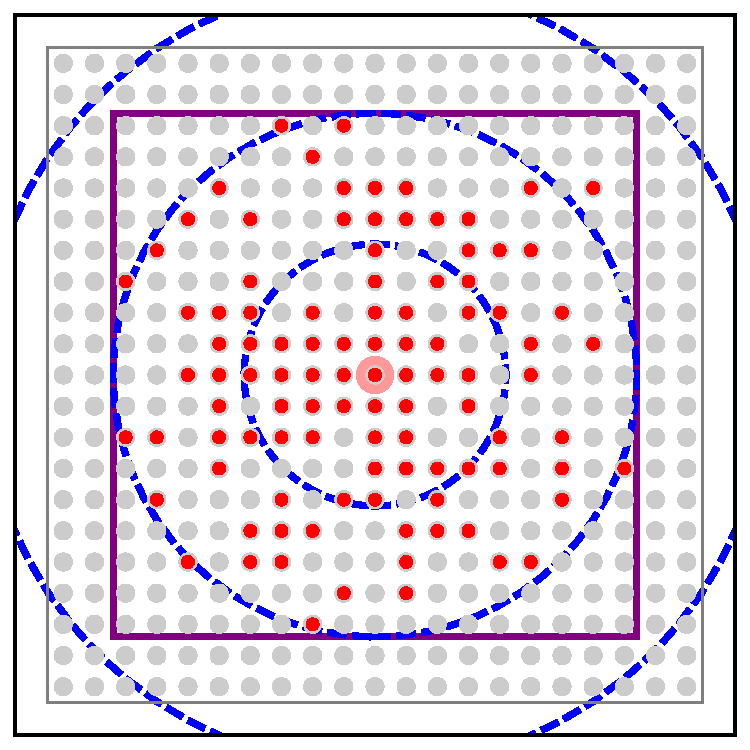
\includegraphics[width=0.6\textwidth]{TopologyExample.pdf}
  \caption[Example of connectivity pattern]{Plot of a layer, with neurons connected to the source node in the center marked in red. The mask is shown in purple, and the blue rings mark $\sigma$, $2 \sigma$ and $3 \sigma$ from the Gaussian kernel function. No nodes outside the mask is connected to the source node. As expected, the fraction of connected nodes is higher close to the source node. Note however, that the actual number of connected nodes is higher between the 1$\sigma$ mark and the 2$\sigma$ mark than between the center and the 1$\sigma$ mark. This is because a greater number of nodes are available further away from the center.}
  \label{fig:topology}
\end{figure} 

It is possible to specify a fixed degree for the driver layer, similar to what is done when using \inline{RandomConvergentConnect} for networks without spatial structure. In this case, each node in the driver layer selects randomly chosen nodes from the pool layer and either connects or not based on the probability given by the kernel, until the number of connections matches the specified degree. This will allow multapses to be formed (unless specifically prohibited). To implement a fixed driver layer degree, only a small change to the parameters given to \inline{ConnectLayers} is needed:
\begin{lstlisting}
conn_specs = {'connection_type': 'convergent', 
              'mask': mask, 'kernel': kernel,
              'number_of_connections': 100,
              'allow_multapses': True}
\end{lstlisting}

Several functions for inspecting different aspects of the network is available, in addition to the plotting functions demonstrated above. All the query functions from the main nest module, such as the \inline{GetTargetNodes} function explained earlier, can also be used on layered networks created with the Topology module. In addition, the topology module provides some extra query functions, such as \inline{FindCenterElement}, \inline{GetTargetPositions}, \inline{Distance}, and \inline{Displacement}. The usage of some of these are demonstrated in the code below, which is a continuation of the previous example. 
\begin{lstlisting}[numbers=left, firstnumber=25]
targets = topo.GetTargetNodes(center_node, target_layer)[0]
distances = topo.Distance(center_node, targets)
import matplotlib.pyplot as plt
plt.figure()
plt.hist(distances, bins=10)
\end{lstlisting}
This will generate a histogram like the one in Figure \ref{fig:inspection}, showing the distribution of distances between the center source node and connected nodes in the target layer.

\begin{figure}[h]
  \centering
  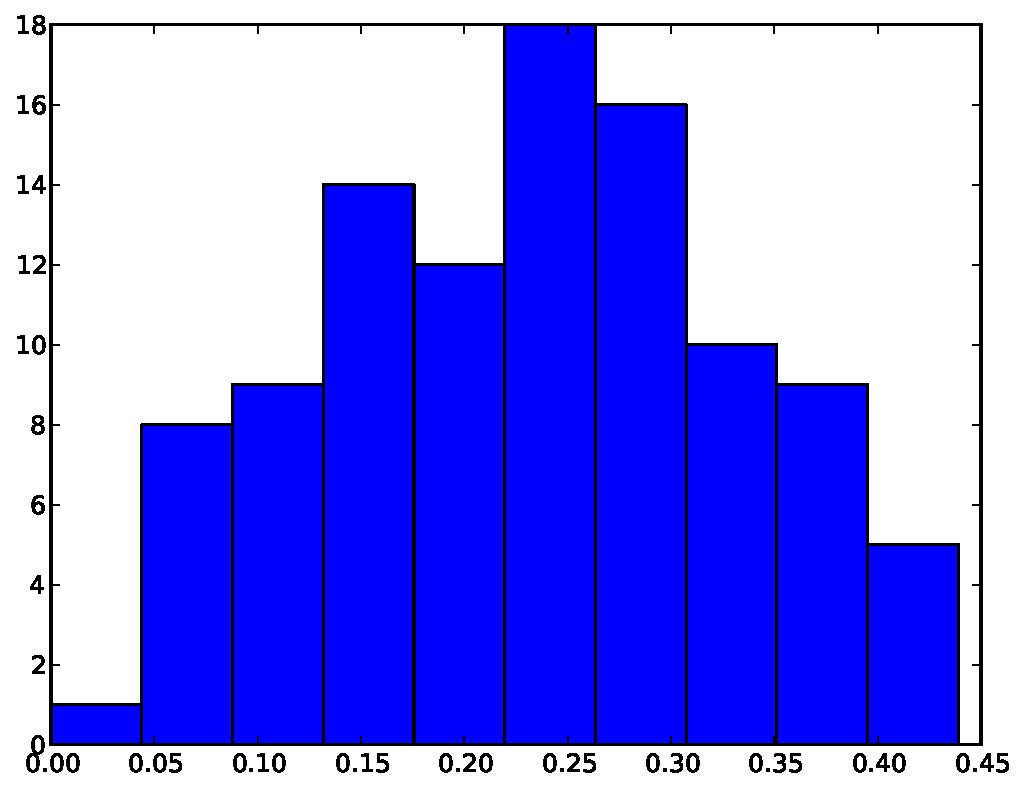
\includegraphics[width=0.6\textwidth]{LayerInspection.pdf}
  \caption[Distribution of distances between source node and connected target nodes]{Distribution of distances between a centered source node and the connected target nodes.}
  \label{fig:inspection}
\end{figure} 



\clearchapter

